% Options for packages loaded elsewhere
\PassOptionsToPackage{unicode}{hyperref}
\PassOptionsToPackage{hyphens}{url}
%
\documentclass[
  12pt,
]{article}
\title{Effective Pest Treament That Protects Pollinators}
\usepackage{etoolbox}
\makeatletter
\providecommand{\subtitle}[1]{% add subtitle to \maketitle
  \apptocmd{\@title}{\par {\large #1 \par}}{}{}
}
\makeatother
\subtitle{\url{https://github.com/shivanikuckreja/CitrolaKuckrejaSaltman_ENV872_EDA_FinalProject/tree/main/Project}}
\author{Sam Saltman, Shivani Kuckreja, Jessica Citrola}
\date{}

\usepackage{amsmath,amssymb}
\usepackage{lmodern}
\usepackage{iftex}
\ifPDFTeX
  \usepackage[T1]{fontenc}
  \usepackage[utf8]{inputenc}
  \usepackage{textcomp} % provide euro and other symbols
\else % if luatex or xetex
  \usepackage{unicode-math}
  \defaultfontfeatures{Scale=MatchLowercase}
  \defaultfontfeatures[\rmfamily]{Ligatures=TeX,Scale=1}
  \setmainfont[]{Times New Roman}
\fi
% Use upquote if available, for straight quotes in verbatim environments
\IfFileExists{upquote.sty}{\usepackage{upquote}}{}
\IfFileExists{microtype.sty}{% use microtype if available
  \usepackage[]{microtype}
  \UseMicrotypeSet[protrusion]{basicmath} % disable protrusion for tt fonts
}{}
\makeatletter
\@ifundefined{KOMAClassName}{% if non-KOMA class
  \IfFileExists{parskip.sty}{%
    \usepackage{parskip}
  }{% else
    \setlength{\parindent}{0pt}
    \setlength{\parskip}{6pt plus 2pt minus 1pt}}
}{% if KOMA class
  \KOMAoptions{parskip=half}}
\makeatother
\usepackage{xcolor}
\IfFileExists{xurl.sty}{\usepackage{xurl}}{} % add URL line breaks if available
\IfFileExists{bookmark.sty}{\usepackage{bookmark}}{\usepackage{hyperref}}
\hypersetup{
  pdftitle={Effective Pest Treament That Protects Pollinators},
  pdfauthor={Sam Saltman, Shivani Kuckreja, Jessica Citrola},
  hidelinks,
  pdfcreator={LaTeX via pandoc}}
\urlstyle{same} % disable monospaced font for URLs
\usepackage[margin=2.54cm]{geometry}
\usepackage{color}
\usepackage{fancyvrb}
\newcommand{\VerbBar}{|}
\newcommand{\VERB}{\Verb[commandchars=\\\{\}]}
\DefineVerbatimEnvironment{Highlighting}{Verbatim}{commandchars=\\\{\}}
% Add ',fontsize=\small' for more characters per line
\usepackage{framed}
\definecolor{shadecolor}{RGB}{248,248,248}
\newenvironment{Shaded}{\begin{snugshade}}{\end{snugshade}}
\newcommand{\AlertTok}[1]{\textcolor[rgb]{0.94,0.16,0.16}{#1}}
\newcommand{\AnnotationTok}[1]{\textcolor[rgb]{0.56,0.35,0.01}{\textbf{\textit{#1}}}}
\newcommand{\AttributeTok}[1]{\textcolor[rgb]{0.77,0.63,0.00}{#1}}
\newcommand{\BaseNTok}[1]{\textcolor[rgb]{0.00,0.00,0.81}{#1}}
\newcommand{\BuiltInTok}[1]{#1}
\newcommand{\CharTok}[1]{\textcolor[rgb]{0.31,0.60,0.02}{#1}}
\newcommand{\CommentTok}[1]{\textcolor[rgb]{0.56,0.35,0.01}{\textit{#1}}}
\newcommand{\CommentVarTok}[1]{\textcolor[rgb]{0.56,0.35,0.01}{\textbf{\textit{#1}}}}
\newcommand{\ConstantTok}[1]{\textcolor[rgb]{0.00,0.00,0.00}{#1}}
\newcommand{\ControlFlowTok}[1]{\textcolor[rgb]{0.13,0.29,0.53}{\textbf{#1}}}
\newcommand{\DataTypeTok}[1]{\textcolor[rgb]{0.13,0.29,0.53}{#1}}
\newcommand{\DecValTok}[1]{\textcolor[rgb]{0.00,0.00,0.81}{#1}}
\newcommand{\DocumentationTok}[1]{\textcolor[rgb]{0.56,0.35,0.01}{\textbf{\textit{#1}}}}
\newcommand{\ErrorTok}[1]{\textcolor[rgb]{0.64,0.00,0.00}{\textbf{#1}}}
\newcommand{\ExtensionTok}[1]{#1}
\newcommand{\FloatTok}[1]{\textcolor[rgb]{0.00,0.00,0.81}{#1}}
\newcommand{\FunctionTok}[1]{\textcolor[rgb]{0.00,0.00,0.00}{#1}}
\newcommand{\ImportTok}[1]{#1}
\newcommand{\InformationTok}[1]{\textcolor[rgb]{0.56,0.35,0.01}{\textbf{\textit{#1}}}}
\newcommand{\KeywordTok}[1]{\textcolor[rgb]{0.13,0.29,0.53}{\textbf{#1}}}
\newcommand{\NormalTok}[1]{#1}
\newcommand{\OperatorTok}[1]{\textcolor[rgb]{0.81,0.36,0.00}{\textbf{#1}}}
\newcommand{\OtherTok}[1]{\textcolor[rgb]{0.56,0.35,0.01}{#1}}
\newcommand{\PreprocessorTok}[1]{\textcolor[rgb]{0.56,0.35,0.01}{\textit{#1}}}
\newcommand{\RegionMarkerTok}[1]{#1}
\newcommand{\SpecialCharTok}[1]{\textcolor[rgb]{0.00,0.00,0.00}{#1}}
\newcommand{\SpecialStringTok}[1]{\textcolor[rgb]{0.31,0.60,0.02}{#1}}
\newcommand{\StringTok}[1]{\textcolor[rgb]{0.31,0.60,0.02}{#1}}
\newcommand{\VariableTok}[1]{\textcolor[rgb]{0.00,0.00,0.00}{#1}}
\newcommand{\VerbatimStringTok}[1]{\textcolor[rgb]{0.31,0.60,0.02}{#1}}
\newcommand{\WarningTok}[1]{\textcolor[rgb]{0.56,0.35,0.01}{\textbf{\textit{#1}}}}
\usepackage{longtable,booktabs,array}
\usepackage{calc} % for calculating minipage widths
% Correct order of tables after \paragraph or \subparagraph
\usepackage{etoolbox}
\makeatletter
\patchcmd\longtable{\par}{\if@noskipsec\mbox{}\fi\par}{}{}
\makeatother
% Allow footnotes in longtable head/foot
\IfFileExists{footnotehyper.sty}{\usepackage{footnotehyper}}{\usepackage{footnote}}
\makesavenoteenv{longtable}
\usepackage{graphicx}
\makeatletter
\def\maxwidth{\ifdim\Gin@nat@width>\linewidth\linewidth\else\Gin@nat@width\fi}
\def\maxheight{\ifdim\Gin@nat@height>\textheight\textheight\else\Gin@nat@height\fi}
\makeatother
% Scale images if necessary, so that they will not overflow the page
% margins by default, and it is still possible to overwrite the defaults
% using explicit options in \includegraphics[width, height, ...]{}
\setkeys{Gin}{width=\maxwidth,height=\maxheight,keepaspectratio}
% Set default figure placement to htbp
\makeatletter
\def\fps@figure{htbp}
\makeatother
\setlength{\emergencystretch}{3em} % prevent overfull lines
\providecommand{\tightlist}{%
  \setlength{\itemsep}{0pt}\setlength{\parskip}{0pt}}
\setcounter{secnumdepth}{5}
\ifLuaTeX
  \usepackage{selnolig}  % disable illegal ligatures
\fi

\begin{document}
\maketitle

\newpage
\tableofcontents 
\newpage
\listoftables 
\newpage
\listoffigures 
\newpage

\hypertarget{rationale-and-research-questions}{%
\section{Rationale and Research
Questions}\label{rationale-and-research-questions}}

\textbf{Pollination is a critical component of agriculture. Bees are
important pollinators. Our research looks to see if there are exposure
methods and chemicals that do not cause significant harm to bees while
eliminating pests. The goal of our research is to determine potential
treatment methods that reduce pests while having little to no impact on
bees.}

Questions:

\begin{enumerate}
\def\labelenumi{\arabic{enumi}.}
\item
  \emph{Is there an exposure type that is more likely to cause mortality
  for bees vs.~non-bee insects?}
\item
  \emph{Are there chemicals that are more likely to cause mortality for
  bees vs.~non-bee insects?}
\end{enumerate}

\newpage

\hypertarget{dataset-information}{%
\section{Dataset Information}\label{dataset-information}}

Data Source: The dataset was pulled from a repository created for
Environmental Data Analytics at Duke University in 2020. The data
collected is from several EPA studies on neonicotinoids and their
effects on insects. The data we will be analyzing is the type of
chemical administered, how it was administered, and how both of these
variables impact insects.

In the wrangling process, we selected the relevant information to our
topic. This includes the chemical type, chemical number, insect species,
lifestage and age of the species, exposure type, the effect of the
exposure and the measurement of the exposure. An example of an exposure
type is giving food to a bee. An example of an effect is mortality, and
the measurement is a more detailed analysis of the effect.

We converted all these selected categorical variables to factors to prep
for analysis. In the next step, we processed two data frames -- oall bee
species and all non-bee species. The split resulted in 2529 non-bee
observations and 1407 bee observations. Lastly we added a mortality
column using an ifelse statement. We did this to run a binomial glm in
our analysis. We coded mortality as 1 and everything else as 0.

\begin{longtable}[]{@{}
  >{\raggedright\arraybackslash}p{(\columnwidth - 2\tabcolsep) * \real{0.44}}
  >{\raggedright\arraybackslash}p{(\columnwidth - 2\tabcolsep) * \real{0.56}}@{}}
\toprule
\begin{minipage}[b]{\linewidth}\raggedright
Detail
\end{minipage} & \begin{minipage}[b]{\linewidth}\raggedright
Description
\end{minipage} \\
\midrule
\endhead
Data Source & EPA ECOTOX Knowledgebase \\
------- & --------- \\
Retrieved From & \url{https://cfpub.epa.gov/ecotox/help.cfm} \\
------- & --------- \\
Variables Used & Chemical Number, Chemical Name, Species Common Name,
Organism Lifestage, Organism Age, Exposure Type, Effect, Effect
Measurement \\
------- & --------- \\
Date Range & 1982-2019 \\
\bottomrule
\end{longtable}

\newpage

\hypertarget{exploratory-analysis}{%
\section{Exploratory Analysis}\label{exploratory-analysis}}

Summary of all species in study

\begin{longtable}[]{@{}lr@{}}
\caption{Species List}\tabularnewline
\toprule
& x \\
\midrule
\endfirsthead
\toprule
& x \\
\midrule
\endhead
Honey Bee & 667 \\
Parasitic Wasp & 285 \\
Buff Tailed Bumblebee & 183 \\
Carniolan Honey Bee & 152 \\
Bumble Bee & 140 \\
Italian Honeybee & 113 \\
Japanese Beetle & 94 \\
Asian Lady Beetle & 76 \\
Euonymus Scale & 75 \\
Wireworm & 69 \\
European Dark Bee & 66 \\
Minute Pirate Bug & 62 \\
Asian Citrus Psyllid & 60 \\
Parastic Wasp & 58 \\
Colorado Potato Beetle & 57 \\
Parasitoid Wasp & 51 \\
Erythrina Gall Wasp & 49 \\
Beetle Order & 47 \\
Snout Beetle Family, Weevil & 47 \\
Sevenspotted Lady Beetle & 46 \\
True Bug Order & 45 \\
Buff-tailed Bumblebee & 39 \\
Aphid Family & 38 \\
Cabbage Looper & 38 \\
Sweetpotato Whitefly & 37 \\
Braconid Wasp & 33 \\
Cotton Aphid & 33 \\
Predatory Mite & 33 \\
Ladybird Beetle Family & 30 \\
Parasitoid & 30 \\
Scarab Beetle & 29 \\
Spring Tiphia & 29 \\
Thrip Order & 29 \\
Ground Beetle Family & 27 \\
Rove Beetle Family & 27 \\
Tobacco Aphid & 27 \\
Chalcid Wasp & 25 \\
Convergent Lady Beetle & 25 \\
Stingless Bee & 25 \\
Spider/Mite Class & 24 \\
Tobacco Flea Beetle & 24 \\
Citrus Leafminer & 23 \\
Ladybird Beetle & 23 \\
Mason Bee & 22 \\
Mosquito & 22 \\
Argentine Ant & 21 \\
Beetle & 21 \\
Flatheaded Appletree Borer & 20 \\
Horned Oak Gall Wasp & 20 \\
Leaf Beetle Family & 20 \\
Potato Leafhopper & 20 \\
Tooth-necked Fungus Beetle & 20 \\
Codling Moth & 19 \\
Black-spotted Lady Beetle & 18 \\
Calico Scale & 18 \\
Fairyfly Parasitoid & 18 \\
Lady Beetle & 18 \\
Minute Parasitic Wasps & 18 \\
Mirid Bug & 18 \\
Mulberry Pyralid & 18 \\
Silkworm & 18 \\
Vedalia Beetle & 18 \\
Araneoid Spider Order & 17 \\
Bee Order & 17 \\
Egg Parasitoid & 17 \\
Insect Class & 17 \\
Moth And Butterfly Order & 17 \\
Oystershell Scale Parasitoid & 17 \\
Hemlock Woolly Adelgid Lady Beetle & 16 \\
Hemlock Wooly Adelgid & 16 \\
Mite & 16 \\
Onion Thrip & 16 \\
Western Flower Thrips & 15 \\
Corn Earworm & 14 \\
Green Peach Aphid & 14 \\
House Fly & 14 \\
Ox Beetle & 14 \\
Red Scale Parasite & 14 \\
Spined Soldier Bug & 14 \\
Armoured Scale Family & 13 \\
Diamondback Moth & 13 \\
Eulophid Wasp & 13 \\
Monarch Butterfly & 13 \\
Predatory Bug & 13 \\
Yellow Fever Mosquito & 13 \\
Braconid Parasitoid & 12 \\
Common Thrip & 12 \\
Eastern Subterranean Termite & 12 \\
Jassid & 12 \\
Mite Order & 12 \\
Pea Aphid & 12 \\
Pond Wolf Spider & 12 \\
Spotless Ladybird Beetle & 11 \\
Glasshouse Potato Wasp & 10 \\
Lacewing & 10 \\
Southern House Mosquito & 10 \\
Two Spotted Lady Beetle & 10 \\
Ant Family & 9 \\
Apple Maggot & 9 \\
(Other) & 670 \\
\bottomrule
\end{longtable}

\newpage

Bar chart comparing exposure type to mortality count of bees. It
initially looked like bees are more likely to die when chemical exposure
comes from consuming food.The other exposure types do not look
particularly significant

\begin{figure}
\centering
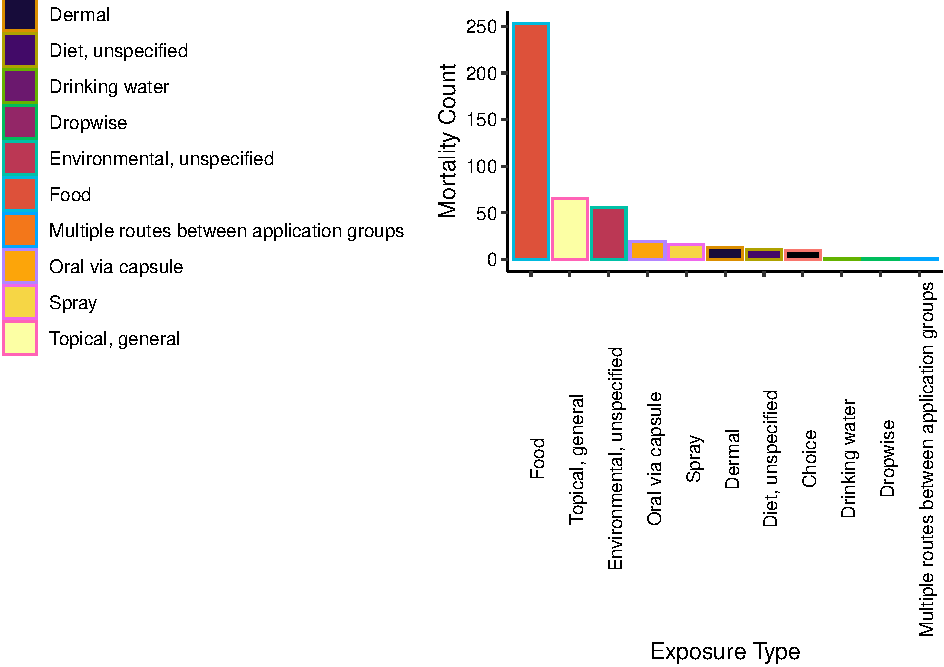
\includegraphics{UpdatedwithModel_files/figure-latex/bee exposure-1.pdf}
\caption{Bee Mortality by Exposure Type}
\end{figure}

\newpage

Bar chart comparing exposure type to mortality count of non-bees.
Exposure from an environmental source appears more lethal to non-bees
species.

\begin{figure}
\centering
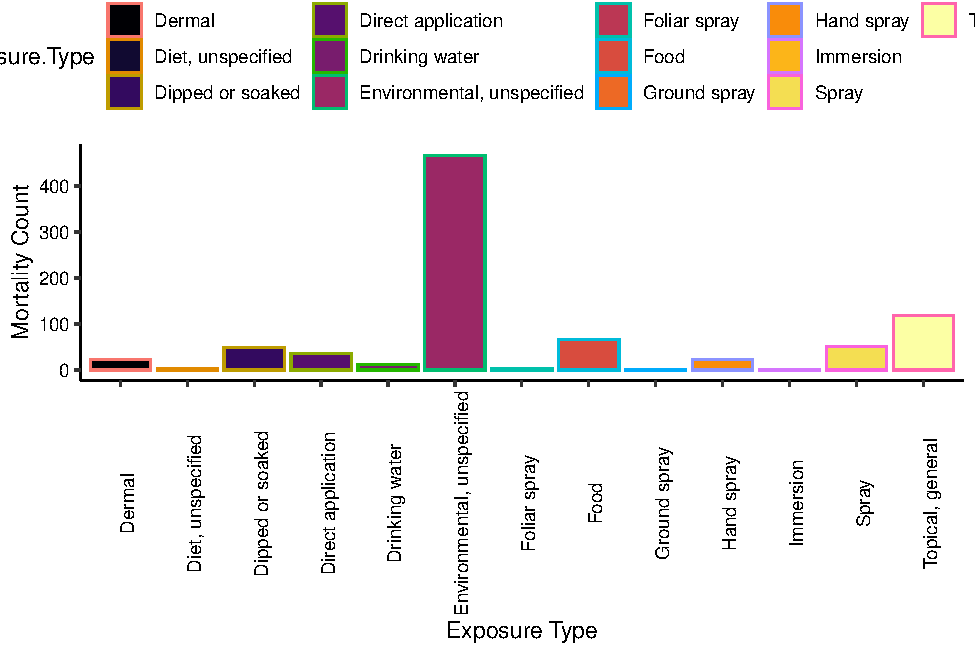
\includegraphics{UpdatedwithModel_files/figure-latex/non bee exposure-1.pdf}
\caption{Non-bee Mortality by Exposure Type}
\end{figure}

\newpage

The next area of exploration was looking into how many bee and non-bee
samples died from exposure to certain chemical compounds. We used the
chemical number as the chemical names are complex.

This bar chart looking at bees suggests that three types of chemical
compounds in this dataset are toxic to bees.

\begin{figure}
\centering
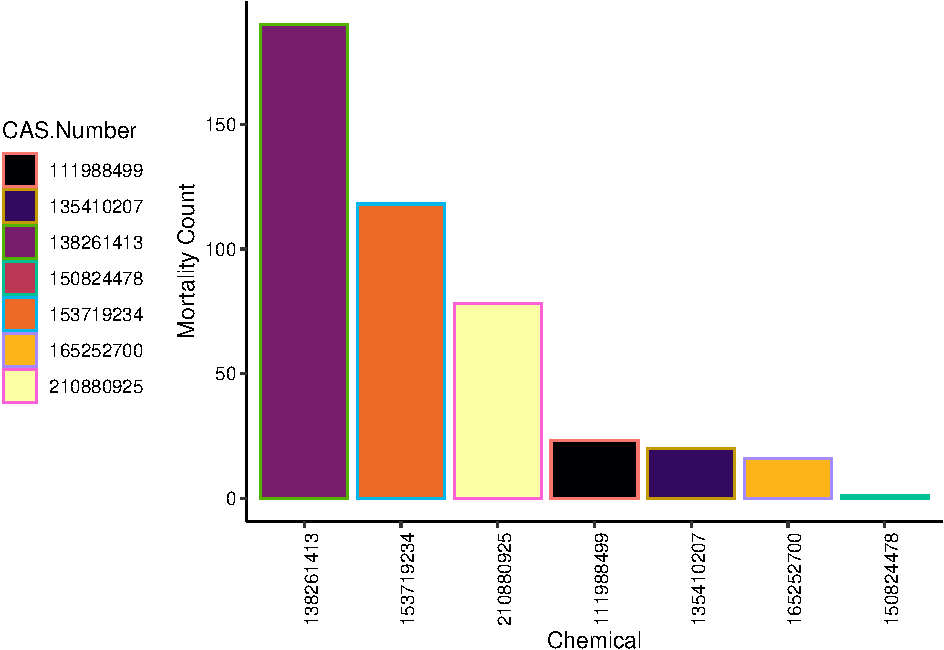
\includegraphics{UpdatedwithModel_files/figure-latex/bee chemical-1.pdf}
\caption{Bee Mortality by Chemical}
\end{figure}

\newpage

This bar chart looking at bees suggests that three types of chemical
compounds in this dataset are toxic to non-bees.

\begin{figure}
\centering
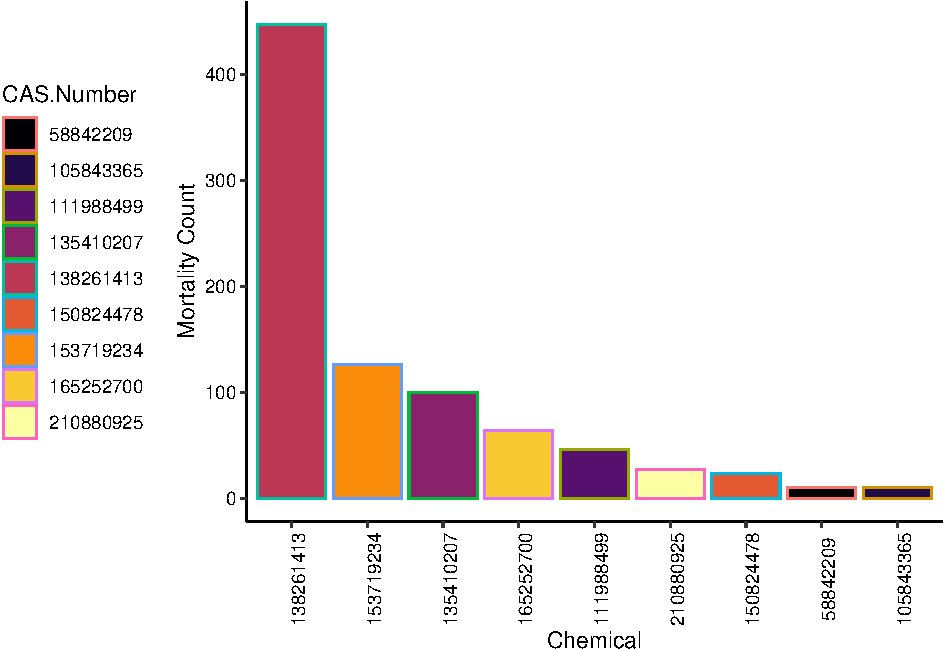
\includegraphics{UpdatedwithModel_files/figure-latex/non bee chemical-1.pdf}
\caption{Non-bee Mortality by Chemical}
\end{figure}

Next we analyze to see if there is any statistical significance
supporting these observations. \newpage

\hypertarget{analysis}{%
\section{Analysis}\label{analysis}}

We ran GLMs to analyze our categorical data. Using the if/else statement
to create the mortality column, we were able to compare mortality
against all other effects. We ran two GLMs for the bee category and two
for the non-bee categories. The two types of GLMs we ran analyzed
mortality against exposure type and mortality against chemical type.To
understand if this regression was a fit, we ran a pseudo regression
using the pR2 function on each GLM as well

\hypertarget{question-1-is-there-an-exposure-type-that-is-more-likely-to-cause-mortality-for-bees-vs.-non-bee-insects}{%
\subsection{Question 1: Is there an exposure type that is more likely to
cause mortality for bees vs.~non-bee
insects?}\label{question-1-is-there-an-exposure-type-that-is-more-likely-to-cause-mortality-for-bees-vs.-non-bee-insects}}

\begin{Shaded}
\begin{Highlighting}[]
\CommentTok{\#Which exposure types have a significant effect (mortality) on bee species?}
\NormalTok{BeeMortalityExposureType}\SpecialCharTok{$}\NormalTok{Mortality }\OtherTok{\textless{}{-}} \FunctionTok{ifelse}\NormalTok{(BeeMortalityExposureType}\SpecialCharTok{$}\NormalTok{Effect}\SpecialCharTok{==}\StringTok{"Mortality"}\NormalTok{, }\DecValTok{1}\NormalTok{, }\DecValTok{0}\NormalTok{) }

\CommentTok{\#Making new column categorical}
\NormalTok{BeeMortalityExposureType}\SpecialCharTok{$}\NormalTok{Mortality }\OtherTok{\textless{}{-}} \FunctionTok{as.factor}\NormalTok{(BeeMortalityExposureType}\SpecialCharTok{$}\NormalTok{Mortality)}

\NormalTok{logit }\OtherTok{\textless{}{-}} \FunctionTok{glm}\NormalTok{(Mortality }\SpecialCharTok{\textasciitilde{}}\NormalTok{ Exposure.Type, }\AttributeTok{data =}\NormalTok{ BeeMortalityExposureType, }\AttributeTok{family =} \StringTok{"binomial"}\NormalTok{)}
\FunctionTok{summary}\NormalTok{(logit)}
\end{Highlighting}
\end{Shaded}

\begin{verbatim}
## 
## Call:
## glm(formula = Mortality ~ Exposure.Type, family = "binomial", 
##     data = BeeMortalityExposureType)
## 
## Deviance Residuals: 
##     Min       1Q   Median       3Q      Max  
## -1.4620  -0.7742  -0.7742   1.1774   1.9728  
## 
## Coefficients:
##                                                          Estimate Std. Error
## (Intercept)                                               -0.5306     0.3985
## Exposure.TypeDermal                                       -0.8747     0.5046
## Exposure.TypeDiet, unspecified                             0.5306     0.5836
## Exposure.TypeDirect application                          -16.0354  1696.7344
## Exposure.TypeDrinking water                               17.0967  2399.5448
## Exposure.TypeDropwise                                     17.0967  2399.5448
## Exposure.TypeEnvironmental, unspecified                    0.1252     0.4343
## Exposure.TypeFood                                         -0.5208     0.4052
## Exposure.TypeGround granular                             -16.0354  1073.1091
## Exposure.TypeHand spray                                  -16.0354  1199.7724
## Exposure.TypeMultiple routes between application groups   -1.2611     1.1513
## Exposure.TypeOral via capsule                             17.0967   550.4935
## Exposure.TypeSpray                                         0.2587     0.5186
## Exposure.TypeTopical, general                              1.1787     0.4512
##                                                         z value Pr(>|z|)   
## (Intercept)                                              -1.331    0.183   
## Exposure.TypeDermal                                      -1.734    0.083 . 
## Exposure.TypeDiet, unspecified                            0.909    0.363   
## Exposure.TypeDirect application                          -0.009    0.992   
## Exposure.TypeDrinking water                               0.007    0.994   
## Exposure.TypeDropwise                                     0.007    0.994   
## Exposure.TypeEnvironmental, unspecified                   0.288    0.773   
## Exposure.TypeFood                                        -1.285    0.199   
## Exposure.TypeGround granular                             -0.015    0.988   
## Exposure.TypeHand spray                                  -0.013    0.989   
## Exposure.TypeMultiple routes between application groups  -1.095    0.273   
## Exposure.TypeOral via capsule                             0.031    0.975   
## Exposure.TypeSpray                                        0.499    0.618   
## Exposure.TypeTopical, general                             2.612    0.009 **
## ---
## Signif. codes:  0 '***' 0.001 '**' 0.01 '*' 0.05 '.' 0.1 ' ' 1
## 
## (Dispersion parameter for binomial family taken to be 1)
## 
##     Null deviance: 1757.6  on 1406  degrees of freedom
## Residual deviance: 1621.4  on 1393  degrees of freedom
## AIC: 1649.4
## 
## Number of Fisher Scoring iterations: 15
\end{verbatim}

\begin{Shaded}
\begin{Highlighting}[]
\CommentTok{\#For every one unit change in Topical, the odds of mortality increase by 1.1787. The P value of topical exposure type is 0.009, and is statistically significant.}
\CommentTok{\#Significance: Total topical samples 99 {-} mortality {-} 65}
\CommentTok{\#Additional data collection is needed on: Exposure through soil contact, drinking}

\CommentTok{\#Pseudo R2}
 \FunctionTok{pR2}\NormalTok{(logit)}
\end{Highlighting}
\end{Shaded}

\begin{verbatim}
## fitting null model for pseudo-r2
\end{verbatim}

\begin{verbatim}
##           llh       llhNull            G2      McFadden          r2ML 
## -810.68616225 -878.77992574  136.18752697    0.07748671    0.09225597 
##          r2CU 
##    0.12934540
\end{verbatim}

\begin{longtable}[]{@{}ll@{}}
\toprule
Exposure Effect on Bees & Pr(\textgreater{} \\
\midrule
\endhead
Topical, general & 0.009 ** \\
\bottomrule
\end{longtable}

\begin{Shaded}
\begin{Highlighting}[]
\CommentTok{\#Which exposure types have a significant effect (mortality) on non bee species?}

\NormalTok{NonBeeMortalityExposure}\SpecialCharTok{$}\NormalTok{Mortality }\OtherTok{\textless{}{-}} \FunctionTok{ifelse}\NormalTok{(NonBeeMortalityExposure}\SpecialCharTok{$}\NormalTok{Effect}\SpecialCharTok{==}\StringTok{"Mortality"}\NormalTok{, }\DecValTok{1}\NormalTok{, }\DecValTok{0}\NormalTok{) }

\CommentTok{\#Making new column categorical}
\NormalTok{NonBeeMortalityExposure}\SpecialCharTok{$}\NormalTok{Mortality }\OtherTok{\textless{}{-}} \FunctionTok{as.factor}\NormalTok{(NonBeeMortalityExposure}\SpecialCharTok{$}\NormalTok{Mortality)}

\NormalTok{logit2 }\OtherTok{\textless{}{-}} \FunctionTok{glm}\NormalTok{(Mortality }\SpecialCharTok{\textasciitilde{}}\NormalTok{ Exposure.Type, }\AttributeTok{data =}\NormalTok{ NonBeeMortalityExposure, }\AttributeTok{family =} \StringTok{"binomial"}\NormalTok{)}
\FunctionTok{summary}\NormalTok{(logit2)}
\end{Highlighting}
\end{Shaded}

\begin{verbatim}
## 
## Call:
## glm(formula = Mortality ~ Exposure.Type, family = "binomial", 
##     data = NonBeeMortalityExposure)
## 
## Deviance Residuals: 
##     Min       1Q   Median       3Q      Max  
## -2.2581  -1.0150  -0.1775   1.2435   2.9497  
## 
## Coefficients:
##                                                              Estimate
## (Intercept)                                                    1.1896
## Exposure.TypeDiet, unspecified                                -0.4964
## Exposure.TypeDipped or soaked                                 -1.3921
## Exposure.TypeDirect application                               -1.9780
## Exposure.TypeDrinking water                                   -1.3437
## Exposure.TypeEnvironmental, unspecified                       -1.5843
## Exposure.TypeFilmcoating                                     -18.7557
## Exposure.TypeFoliar spray                                     -5.5269
## Exposure.TypeFood                                             -0.4814
## Exposure.TypeGround granular                                 -18.7557
## Exposure.TypeGround spray                                     -5.3327
## Exposure.TypeHand spray                                       -2.8824
## Exposure.TypeImmersion                                        16.3765
## Exposure.TypeMisted                                          -18.7557
## Exposure.TypeMultiple routes within environmental exposures  -18.7557
## Exposure.TypePresent in soil                                 -18.7557
## Exposure.TypeSpray                                            -2.5710
## Exposure.TypeTopical, general                                  1.2785
## Exposure.TypeWatered                                         -18.7557
##                                                             Std. Error z value
## (Intercept)                                                     0.4317   2.756
## Exposure.TypeDiet, unspecified                                  0.9676  -0.513
## Exposure.TypeDipped or soaked                                   0.4727  -2.945
## Exposure.TypeDirect application                                 0.4774  -4.144
## Exposure.TypeDrinking water                                     0.5840  -2.301
## Exposure.TypeEnvironmental, unspecified                         0.4358  -3.635
## Exposure.TypeFilmcoating                                     3956.1804  -0.005
## Exposure.TypeFoliar spray                                       0.8324  -6.640
## Exposure.TypeFood                                               0.4812  -1.000
## Exposure.TypeGround granular                                  273.0027  -0.069
## Exposure.TypeGround spray                                       1.0965  -4.864
## Exposure.TypeHand spray                                         0.4877  -5.911
## Exposure.TypeImmersion                                       3956.1804   0.004
## Exposure.TypeMisted                                          1398.7210  -0.013
## Exposure.TypeMultiple routes within environmental exposures  2797.4420  -0.007
## Exposure.TypePresent in soil                                 2284.1018  -0.008
## Exposure.TypeSpray                                              0.4592  -5.599
## Exposure.TypeTopical, general                                   0.5430   2.355
## Exposure.TypeWatered                                         1142.0510  -0.016
##                                                             Pr(>|z|)    
## (Intercept)                                                 0.005855 ** 
## Exposure.TypeDiet, unspecified                              0.607926    
## Exposure.TypeDipped or soaked                               0.003227 ** 
## Exposure.TypeDirect application                             3.42e-05 ***
## Exposure.TypeDrinking water                                 0.021404 *  
## Exposure.TypeEnvironmental, unspecified                     0.000278 ***
## Exposure.TypeFilmcoating                                    0.996217    
## Exposure.TypeFoliar spray                                   3.14e-11 ***
## Exposure.TypeFood                                           0.317121    
## Exposure.TypeGround granular                                0.945227    
## Exposure.TypeGround spray                                   1.15e-06 ***
## Exposure.TypeHand spray                                     3.41e-09 ***
## Exposure.TypeImmersion                                      0.996697    
## Exposure.TypeMisted                                         0.989301    
## Exposure.TypeMultiple routes within environmental exposures 0.994651    
## Exposure.TypePresent in soil                                0.993448    
## Exposure.TypeSpray                                          2.16e-08 ***
## Exposure.TypeTopical, general                               0.018538 *  
## Exposure.TypeWatered                                        0.986897    
## ---
## Signif. codes:  0 '***' 0.001 '**' 0.01 '*' 0.05 '.' 0.1 ' ' 1
## 
## (Dispersion parameter for binomial family taken to be 1)
## 
##     Null deviance: 3233.2  on 2528  degrees of freedom
## Residual deviance: 2540.4  on 2510  degrees of freedom
## AIC: 2578.4
## 
## Number of Fisher Scoring iterations: 16
\end{verbatim}

\begin{Shaded}
\begin{Highlighting}[]
\CommentTok{\#Dipped or soaked, Direct application, Environmental{-} unspecified, Foliar spray, Ground spray, Hand spray, Spray, and Topical, general are all significant }
\CommentTok{\#Plenty of samples for non{-}bees {-} correlations  }
\CommentTok{\#Conclusion: Spray could be an effective anthropogenic exposure technique to eliminate pests and preserve bees. Direct application like topical techniques should be avoided as they significantly harm all species. There appears to be environmental exposure types that can promote desired effect as well.}

\CommentTok{\#Pseudo R2}
 \FunctionTok{pR2}\NormalTok{(logit2)}
\end{Highlighting}
\end{Shaded}

\begin{verbatim}
## fitting null model for pseudo-r2
\end{verbatim}

\begin{verbatim}
##           llh       llhNull            G2      McFadden          r2ML 
## -1270.1751454 -1616.5870098   692.8237287     0.2142859     0.2396312 
##          r2CU 
##     0.3321160
\end{verbatim}

\begin{longtable}[]{@{}ll@{}}
\toprule
Non-Bee Exposure Type & Pr(\textgreater{} \\
\midrule
\endhead
Dipped or soaked & 0.003227 \\
Direct application & 3.42e-05 \\
Drinking water & 0.021404 \\
Environmental, unspecified & 0.000278 \\
Foliar spray & 3.14e-11 \\
Ground spray & 1.15e-06 \\
Hand spray & 3.41e-09 \\
Spray & 2.16e-08 \\
Topical, general & 0.018538 \\
\bottomrule
\end{longtable}

\hypertarget{question-2-are-there-chemicals-that-are-more-likely-to-cause-mortality-for-bees-vs.-non-bee-insects}{%
\subsection{Question 2: Are there chemicals that are more likely to
cause mortality for bees vs.~non-bee
insects?}\label{question-2-are-there-chemicals-that-are-more-likely-to-cause-mortality-for-bees-vs.-non-bee-insects}}

\begin{Shaded}
\begin{Highlighting}[]
\CommentTok{\#Which chemical types have a significant effect (mortality) on bee species?}

\NormalTok{logit3 }\OtherTok{\textless{}{-}} \FunctionTok{glm}\NormalTok{(Mortality }\SpecialCharTok{\textasciitilde{}}\NormalTok{ CAS.Number, }\AttributeTok{data =}\NormalTok{ BeeMortalityExposureType, }\AttributeTok{family =} \StringTok{"binomial"}\NormalTok{)}
\FunctionTok{summary}\NormalTok{(logit3)}
\end{Highlighting}
\end{Shaded}

\begin{verbatim}
## 
## Call:
## glm(formula = Mortality ~ CAS.Number, family = "binomial", data = BeeMortalityExposureType)
## 
## Deviance Residuals: 
##     Min       1Q   Median       3Q      Max  
## -1.5453  -0.7585  -0.7585   1.2286   1.7080  
## 
## Coefficients:
##                     Estimate Std. Error z value Pr(>|z|)    
## (Intercept)           0.8329     0.3788   2.199 0.027885 *  
## CAS.Number135410207  -2.0268     0.4568  -4.437 9.10e-06 ***
## CAS.Number138261413  -1.9315     0.3879  -4.979 6.39e-07 ***
## CAS.Number150824478  11.7332   324.7439   0.036 0.971178    
## CAS.Number153719234  -0.9526     0.3993  -2.385 0.017062 *  
## CAS.Number165252700  -1.4276     0.4904  -2.911 0.003599 ** 
## CAS.Number210880925  -1.5066     0.4035  -3.734 0.000189 ***
## ---
## Signif. codes:  0 '***' 0.001 '**' 0.01 '*' 0.05 '.' 0.1 ' ' 1
## 
## (Dispersion parameter for binomial family taken to be 1)
## 
##     Null deviance: 1757.6  on 1406  degrees of freedom
## Residual deviance: 1689.6  on 1400  degrees of freedom
## AIC: 1703.6
## 
## Number of Fisher Scoring iterations: 11
\end{verbatim}

\begin{Shaded}
\begin{Highlighting}[]
 \CommentTok{\#Need more data on 58842209 105843365 and 58842209, 150824478}
 \CommentTok{\# Every other chemical is statistically significant {-} 111988499 135410207 138261413  153719234 165252700 210880925 }

\CommentTok{\#Pseudo R2}
 \FunctionTok{pR2}\NormalTok{(logit3)}
\end{Highlighting}
\end{Shaded}

\begin{verbatim}
## fitting null model for pseudo-r2
\end{verbatim}

\begin{verbatim}
##           llh       llhNull            G2      McFadden          r2ML 
## -844.79573614 -878.77992574   67.96837921    0.03867201    0.04715907 
##          r2CU 
##    0.06611832
\end{verbatim}

\begin{longtable}[]{@{}ll@{}}
\toprule
Chemical Effect on Bees & Pr(\textgreater{} \\
\midrule
\endhead
135410207 & 9.10e-06 *** \\
138261413 & 6.39e-07 *** \\
153719234 & 0.017062 * \\
165252700 & 0.003599 ** \\
210880925 & 0.000189 *** \\
\bottomrule
\end{longtable}

\begin{Shaded}
\begin{Highlighting}[]
\CommentTok{\#Which exposure types have a significant effect (mortality) on non bee species?}

\NormalTok{logit4 }\OtherTok{\textless{}{-}} \FunctionTok{glm}\NormalTok{(Mortality }\SpecialCharTok{\textasciitilde{}}\NormalTok{ CAS.Number, }\AttributeTok{data =}\NormalTok{ NonBeeMortalityExposure, }\AttributeTok{family =} \StringTok{"binomial"}\NormalTok{)}
\FunctionTok{summary}\NormalTok{(logit4)}
\end{Highlighting}
\end{Shaded}

\begin{verbatim}
## 
## Call:
## glm(formula = Mortality ~ CAS.Number, family = "binomial", data = NonBeeMortalityExposure)
## 
## Deviance Residuals: 
##     Min       1Q   Median       3Q      Max  
## -1.5928  -0.8379  -0.8379   1.2907   1.9027  
## 
## Coefficients:
##                       Estimate Std. Error z value Pr(>|z|)
## (Intercept)          1.557e+01  4.602e+02   0.034    0.973
## CAS.Number105843365  1.448e-09  6.509e+02   0.000    1.000
## CAS.Number111988499 -1.507e+01  4.602e+02  -0.033    0.974
## CAS.Number135410207 -1.583e+01  4.602e+02  -0.034    0.973
## CAS.Number138261413 -1.643e+01  4.602e+02  -0.036    0.972
## CAS.Number150824478 -1.463e+01  4.602e+02  -0.032    0.975
## CAS.Number153719234 -1.615e+01  4.602e+02  -0.035    0.972
## CAS.Number165252700 -1.580e+01  4.602e+02  -0.034    0.973
## CAS.Number210880925 -1.720e+01  4.602e+02  -0.037    0.970
## 
## (Dispersion parameter for binomial family taken to be 1)
## 
##     Null deviance: 3233.2  on 2528  degrees of freedom
## Residual deviance: 3091.8  on 2520  degrees of freedom
## AIC: 3109.8
## 
## Number of Fisher Scoring iterations: 14
\end{verbatim}

\begin{Shaded}
\begin{Highlighting}[]
\CommentTok{\#There is no chemical that is effective at eliminating all non{-}bee species. }
\CommentTok{\#Conclusion {-} exposure mechanism of chemical is a more reliable factor at understanding mortality than chemical itself. Bees do not respond well to any of the adminstered chemicals. Any treatment should focus on using the chemicals in ways that are ineffective at exposing bees and effective at exposing nonbees}

\CommentTok{\#Pseudo R2}
 \FunctionTok{pR2}\NormalTok{(logit4)}
\end{Highlighting}
\end{Shaded}

\begin{verbatim}
## fitting null model for pseudo-r2
\end{verbatim}

\begin{verbatim}
##           llh       llhNull            G2      McFadden          r2ML 
## -1.545888e+03 -1.616587e+03  1.413983e+02  4.373360e-02  5.437649e-02 
##          r2CU 
##  7.536291e-02
\end{verbatim}

\begin{longtable}[]{@{}ll@{}}
\toprule
Chemical Effect on Non-Bees & Pr(\textgreater{} \\
\midrule
\endhead
Chemical & None \\
\bottomrule
\end{longtable}

\newpage

\hypertarget{summary-and-conclusions}{%
\section{Summary and Conclusions}\label{summary-and-conclusions}}

\newpage

\hypertarget{references}{%
\section{References}\label{references}}

\textless add references here if relevant, otherwise delete this
section\textgreater{}

\end{document}
